\documentclass[a4paper, 12pt]{article}
\usepackage[T2A]{fontenc}
\usepackage[utf8]{inputenc}
\usepackage[english,russian]{babel}
\usepackage{amsmath, amsfonts, amssymb, amsthm, mathtools, misccorr, indentfirst}
\author{Нехаев Александр Сергеевич\\654 группа}
\title{Газоразрядный стабилизатор напряжения}
\date{2 марта 2018 г.}
\begin{document}
\begin{titlepage}
\begin{center}
Московский Физико-Технический Институт\\
(государственный университет)\\
\vspace{0.5cm}
Кафедра вакуумной электроники\\
\vspace{1.5cm}
\huge
Газоразрядный стабилизатор напряжения\\
\vspace{0.5cm}
\small
Лабораторная работа по курсу \textit{Вакуумная электроника}\\
\vspace{5cm}
\end{center}
\begin{flushright}
Работу выполнил:\\
Нехаев Александр Сергеевич\\
654 группа\\
2 марта 2018 г.
\end{flushright}
\begin{center}
\vspace{5.7 cm}
Долгопрудный\\
2018
\end{center}
\end{titlepage}
\pagenumbering{gobble}
\newpage
\tableofcontents
\pagenumbering{arabic}
\newpage
\section{Цель работы}
Рассмотреть и изучить самостоятельный тлеющий разряд и основанное на его свойствах явление стабилизации напряжения(стабиловольта). Исследовать характеристики стабиловольта, а также ознакомиться с основными физическими явлениями, обуславливающими прохождение электрического тока в газах.
\section{Теоретические основы}
Газовым разрядом в широком смысле слова называется всякое прохождение электрического тока через газы. Газовые разряды бывают несамостоятельные и самостоятельные. Носители тока в несамостоятельных разрядах возникают за счет внешней ионизации, не связанной с напряжением, приложенным к электродам газового промежутка. С прекращением ионизации такие разряды исчезают. Самостоятельные газовые разряды возникают в результате ионизации молекул и атомов самого газа, и их течение не зависит от внешней ионизации. В данной работе мы рассматриваем только тлеющий разряд и основанное на его свойствах явление стабилизации напряжения.\par
Рассмотрим основные особенности тлеющего разряда. Переход от несамостоятельного разряда к самостоятельному обычно сопровождается резким увеличением силы тока и внезапным появлением течения газа. Однако если внешнее сопротивление очень велико (порядка $10^6$ Ом), переход от несамостоятельного разряда к самостоятельному происходит постепенно, и можно наблюдать переходную форму разряда. При напряжении, равном напряжению зажигания, около анода появляется слабое свечение. При увеличении тока начинается искажение поля пространственными зарядами, а свечение начинает распространяться по направлению к катоду. При дальнейшем увеличении силы тока свечение газа начинает распадаться на характерные для тлеющего разряда части, а падение потенциала в трубке сосредоточивается в катодных частях разряда. Обычно тлеющий разряд возникает при низких давлениях (от сотых долей до десятков мм рт. ст.).\par
\begin{figure}[h!]
	\centering
	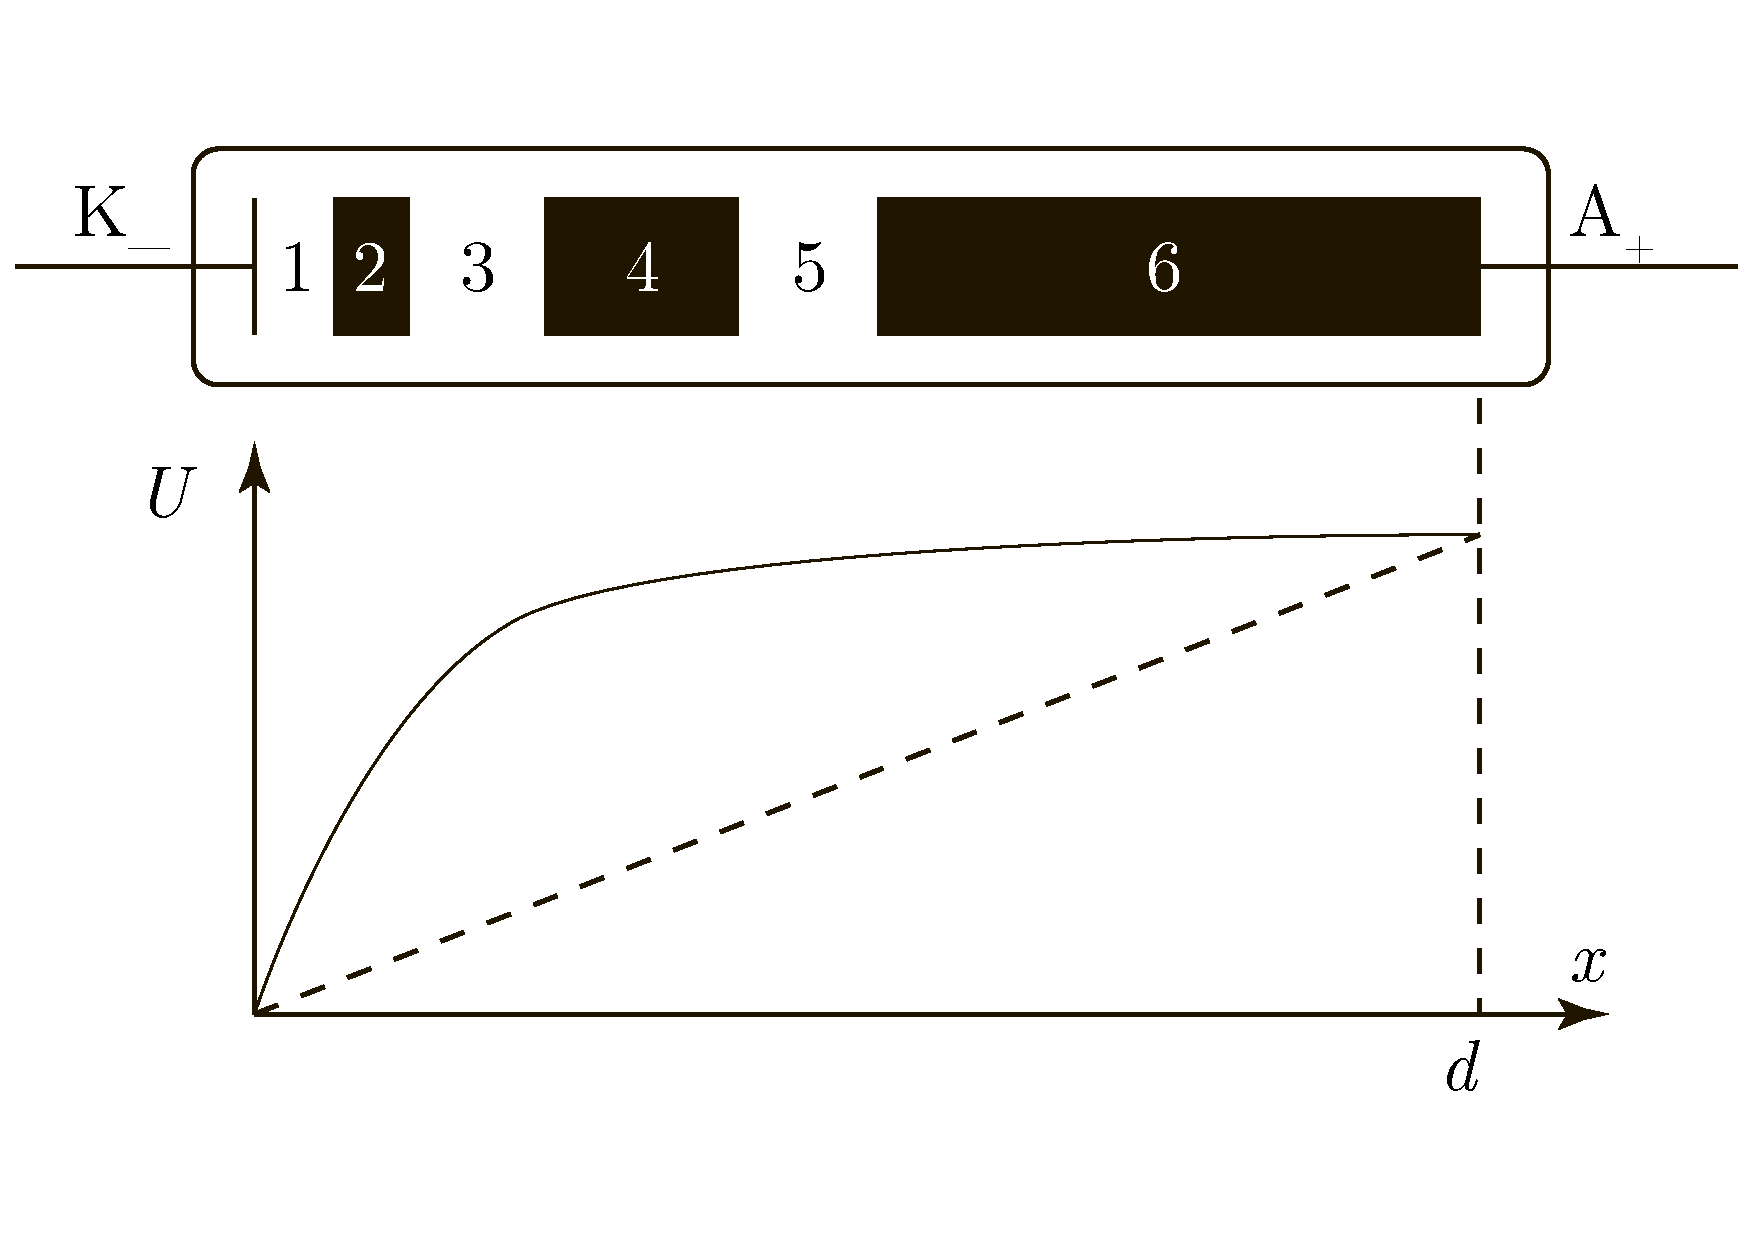
\includegraphics[scale=0.4]{Graph7.pdf}
	\caption{Области тлеющего разряда и распределение потенциала в газоразрядной трубке}
	\label{fig:Graph7}
\end{figure}
\par
Название областей на рис. \ref{fig:Graph7}:
\begin{enumerate}
		\item астоново темное пространство;
		\item катодная светящаяся пленка;
		\item катодное темное пространство;
		\item тлеющее свечение;
		\item темное фарадеево пространство;
		\item область положительного столба (плазма).
\end{enumerate}
\par
Стабиловольт представляет собой газоразрядный прибор с холодным катодом. Простейший стабиловольт состоит из двух электродов, помещенных в баллон с инертным газом при пониженном давлении. Действие прибора основано на использовании тлеющего газового разряда с нормальным падением потенциала. В начале разряда используется только часть поверхности катода, а при увеличении тока рабочая поверхность катода увеличивается при почти неизменных напряжениях на приборе и плотности тока.\par
\newpage
\section{Экспериментальная установка}
Принципиальная схема лабораторной вакуумной установки представлена на рис. \ref{fig:MyGraph6}.
\begin{figure}[h!]
	\centering
	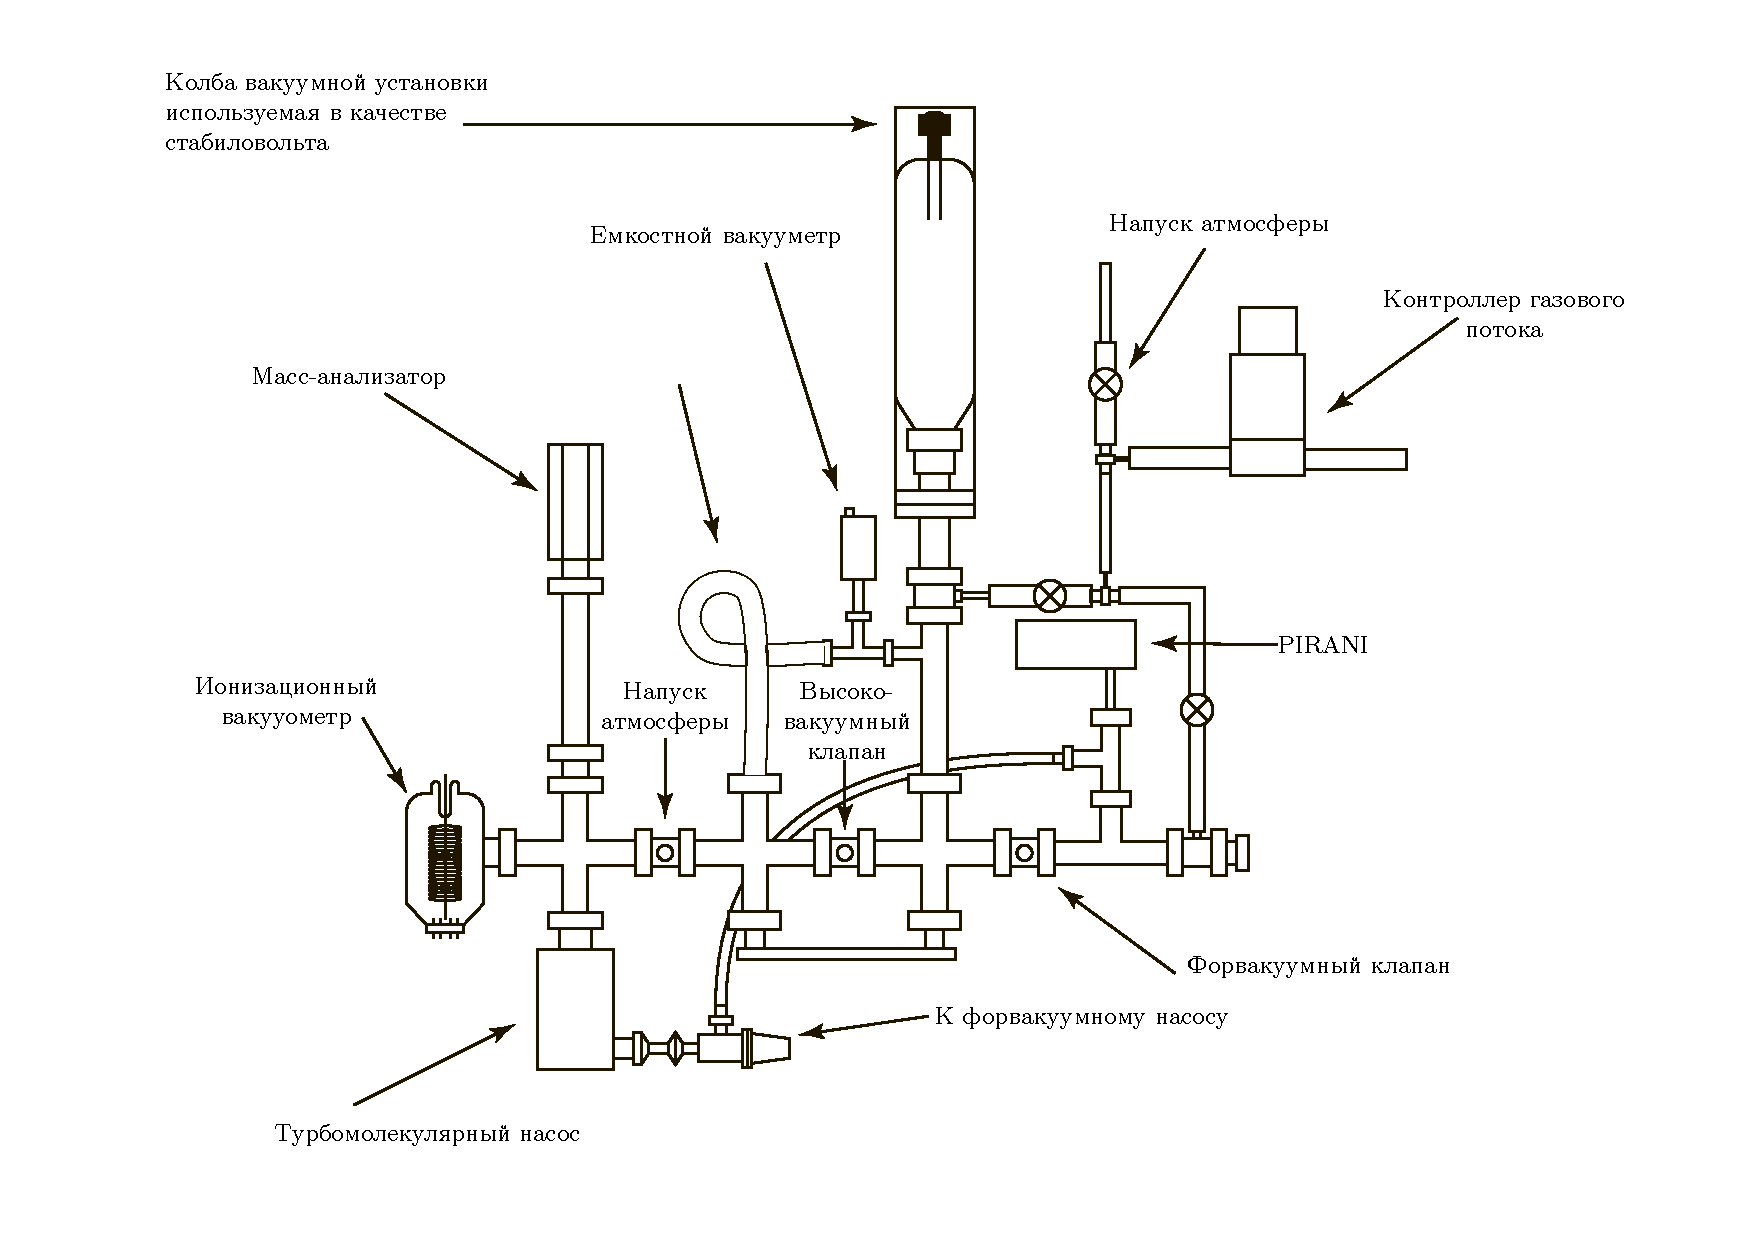
\includegraphics[scale=0.4]{MyGraph6.pdf}
	\caption{Схема лабораторной установки}
	\label{fig:MyGraph6}
\end{figure}
\section{Практическая часть}
\subsection{Задание 1}
Снимем семейство вольтамперных характеристик стабиловольта при нормальной полярности электродов, повышая и понижая входное напряжение, используя в качестве параметра давление газа в приборе. В данном эксперименте в качестве газа используем воздух.
\par
\begin{table}[h!]
\centering
\begin{tabular}{|c|c|c|}
\hline
$v_\text{н}\text{, см}^3\text{/c}$ & $P\text{, торр}$ & $U_3\text{, кВ}$ \\
\hline
100 & 1.36 & 0.74 \\
\hline
50 & 0.78 & 0.66 \\
\hline
25 & 0.446 & 0.63 \\
\hline
12.5 & 0.265 & 0.65 \\
\hline
20 & 0.367 & 0.64 \\
\hline
30 & 0.58 & 0.64 \\
\hline
27.5 & 0.481 & 0.64 \\
\hline
10 & 0.236 & 0.65 \\
\hline
5 & 0.139 & 0.65 \\
\hline
\end{tabular}
\caption{Зависимость для воздуха $U_3\left(P\right)$}
\end{table}
Построим график зависимости $U_3\left(P\right)$:
\begin{figure}[h!]
\centering
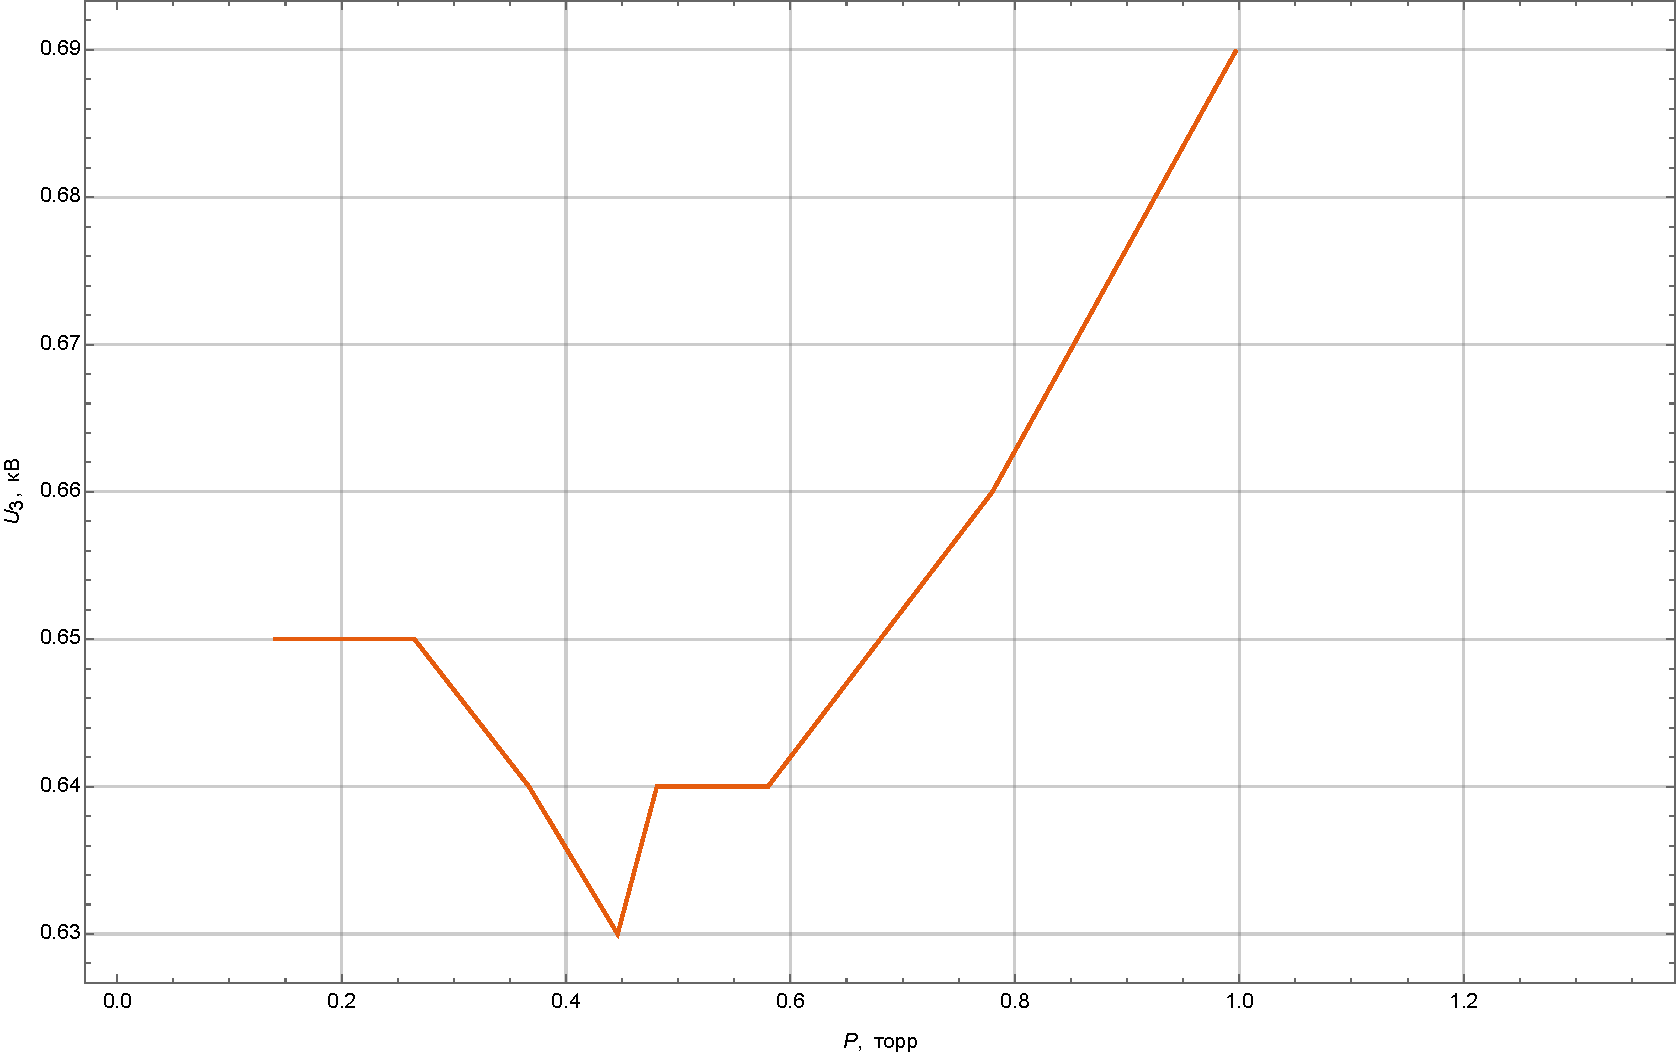
\includegraphics[scale=0.42]{MyGraph1.pdf}
\caption{График зависимости $U_3\left(P\right)$}
\label{fig:exp1}
\end{figure}
\par
Снимем ВАХ для воздуха $f=I\left(U\right)$ при тех же условиях.
\begin{table}[h!]
\centering
\begin{tabular}{|c|c|}
\hline
$I$, А & $U$, кВ \\
\hline
19 & 0.63 \\
\hline
16.94 & 0.63 \\
\hline
15.08 & 0.64 \\
\hline
13.03 & 0.64 \\
\hline
10.98 & 0.65 \\
\hline
9.03 & 0.65 \\
\hline
6.99 & 0.66 \\
\hline
4.99 & 0.68 \\
\hline
3.02 & 0.7 \\
\hline
1.03 & 0.71 \\
\hline
\end{tabular}
\caption{ВАХ для воздуха $I\left(U\right)$}
\end{table}
\par
Построим график для ВАХ воздуха:
\begin{figure}[h!]
\centering
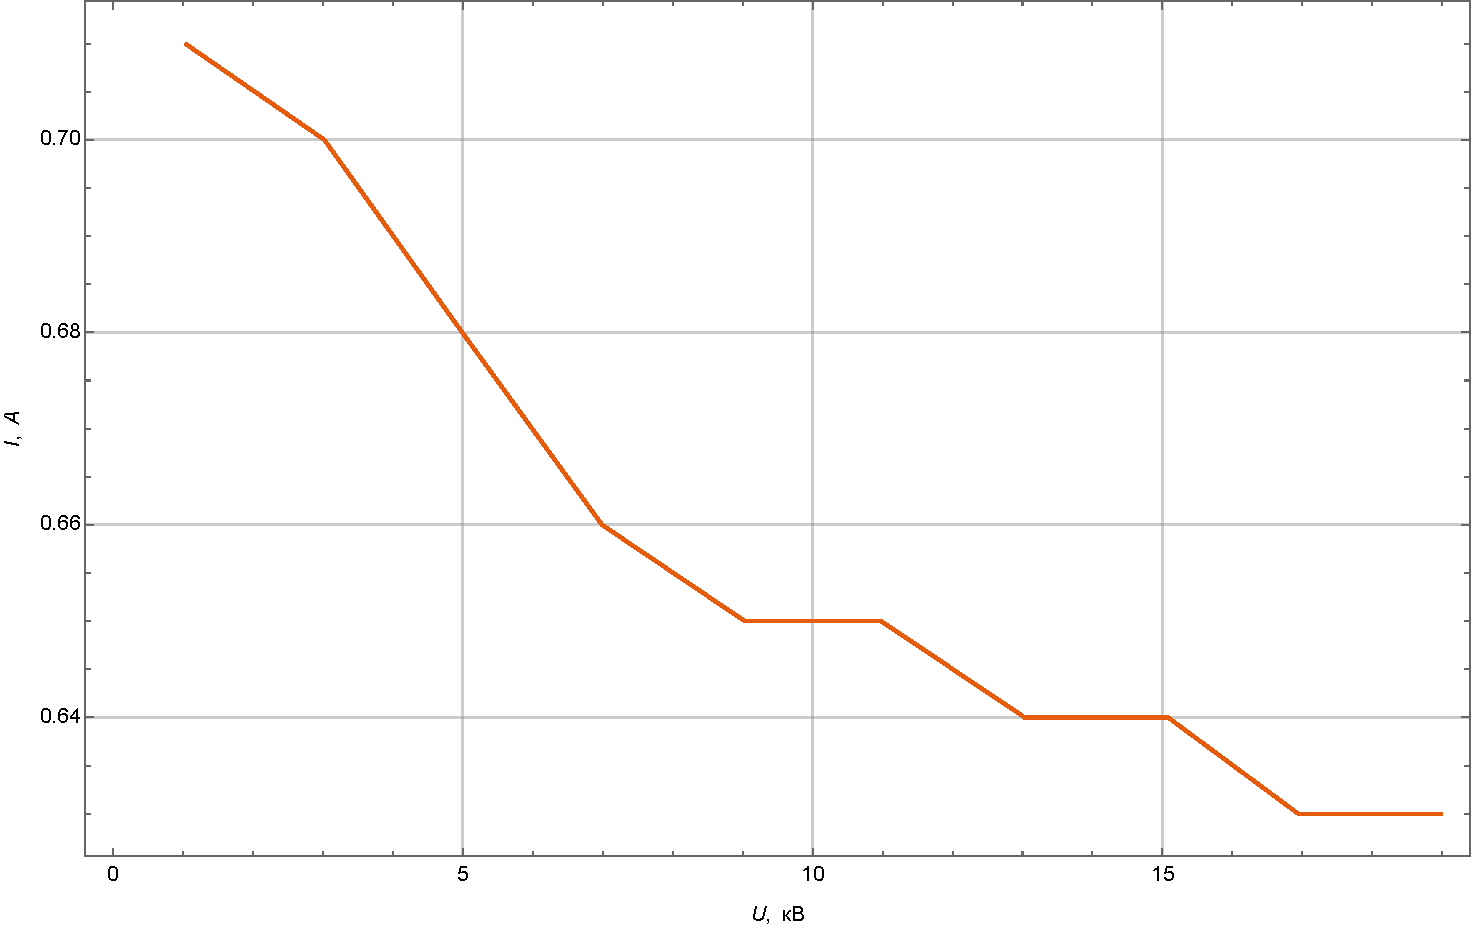
\includegraphics[scale=0.5]{MyGraph2.pdf}
\caption{График зависимости $I\left(U\right)$ при 25 $\frac{\text{см}^3}{\text{с}}$}
\label{fig:exp2}
\end{figure}
\newpage
\subsection{Задание 2}
Снимем аналогичные характеристики для смеси газов: воздуха и аргона.
\begin{table}[h!]
\centering
\begin{tabular}{|c|c|c|}
\hline
$v_\text{н}\text{, см}^3\text{/c}$ & $P\text{, торр}$ & $U_3\text{, кВ}$ \\
\hline
100 & 1.32 & 0.48 \\
\hline
50 & 0.759 & 0.47 \\
\hline
25 & 0.421 & 0.42 \\
\hline
12.5 & 0.249 & 0.41 \\
\hline
6.5 & 0.154 & 0.43 \\
\hline
11 & 0.215 & 0.42 \\
\hline
5 & 0.124 & 0.44 \\
\hline
20 & 0.323 & 0.42 \\
\hline
17 & 0.292 & 0.41 \\
\hline
15 & 0.268 & 0.41 \\
\hline
\end{tabular}
\caption{Зависимость для смеси воздуха и аргона $U_3\left(P\right)$}
\end{table}
\begin{figure}[h!]
\centering
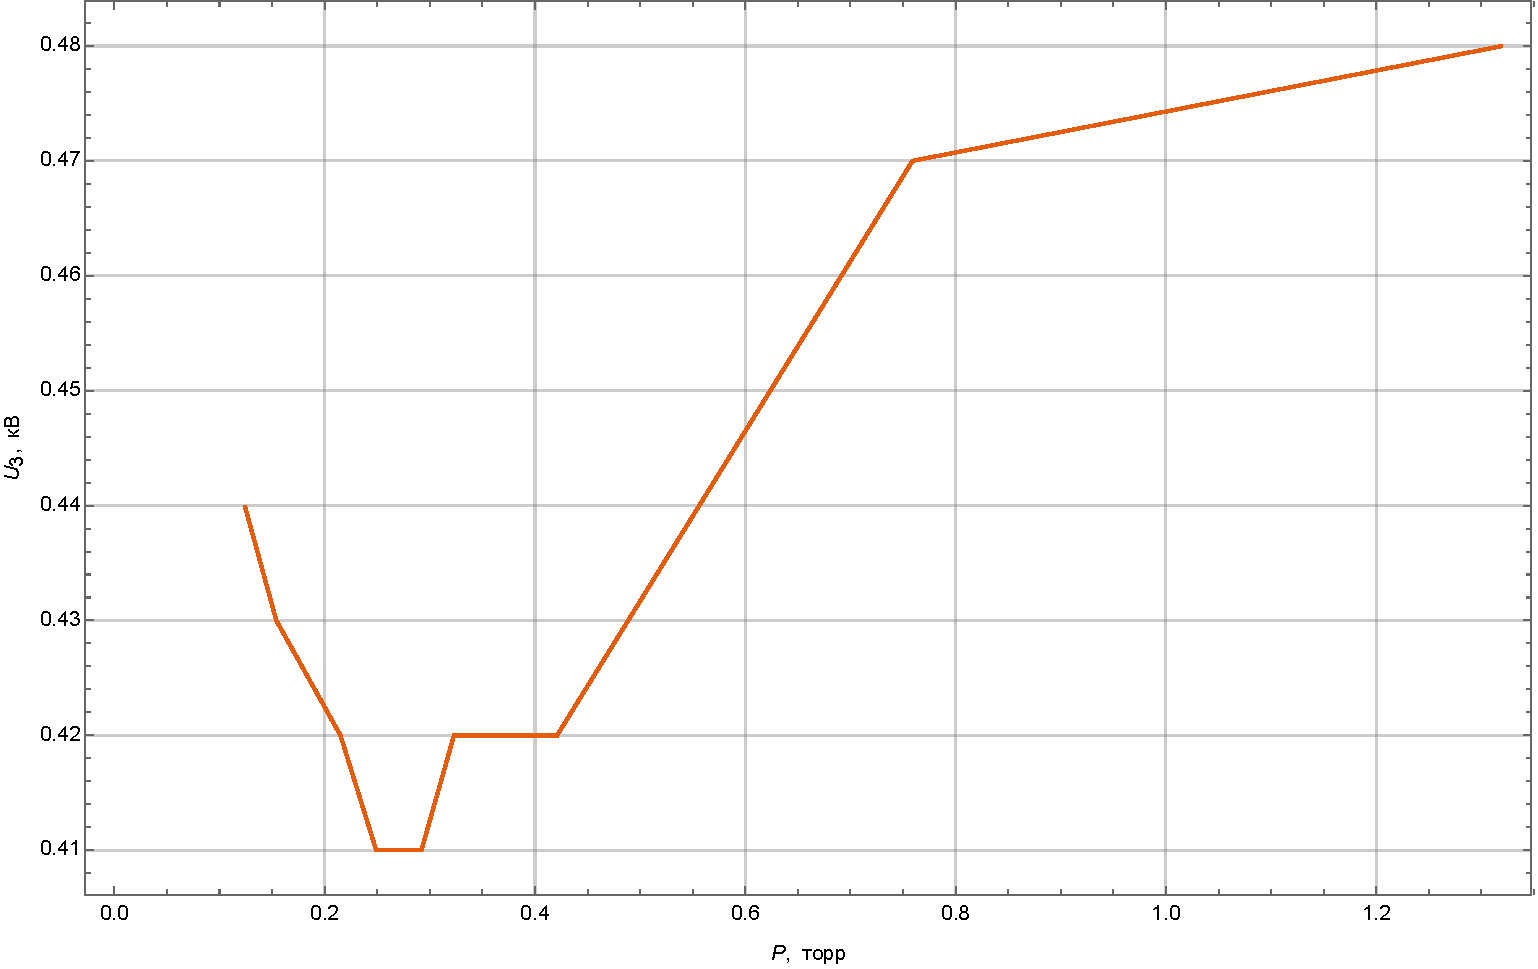
\includegraphics[scale=0.5]{MyGraph3.pdf}
\caption{График зависимости $U_3\left(P\right)$}
\end{figure}
\par
Снимем зависимость ВАХ для смеси аргона и воздуха.
\begin{table}[h!]
\centering
	\begin{tabular}{|c|c|}
\hline
 $I$, А & $U$, кВ \\
\hline
 19.03 & 0.41 \\
\hline
 17.07 & 0.42 \\
\hline
 15.02 & 0.42 \\
\hline
 12.99 & 0.42 \\
\hline
 11.08 & 0.42 \\
\hline
 9.01 & 0.46 \\
\hline
 7.02 & 0.48 \\
\hline
 5.01 & 0.48 \\
\hline
 3. & 0.49 \\
\hline
 1.07 & 0.5 \\
\hline
 0.5 & 0.49 \\
\hline
\end{tabular}
\caption{ВАХ для смеси воздуха и аргона $I\left(U\right)$}
\end{table}
\newpage
\subsection{Задание 3}
Сравним характеристики в случае воздуха и в случае воздуха, перемешанного с Аргоном. Сравнение графиков приведено на рис. \ref{fig:Graph5}
\begin{figure}[h!]
	\centering
	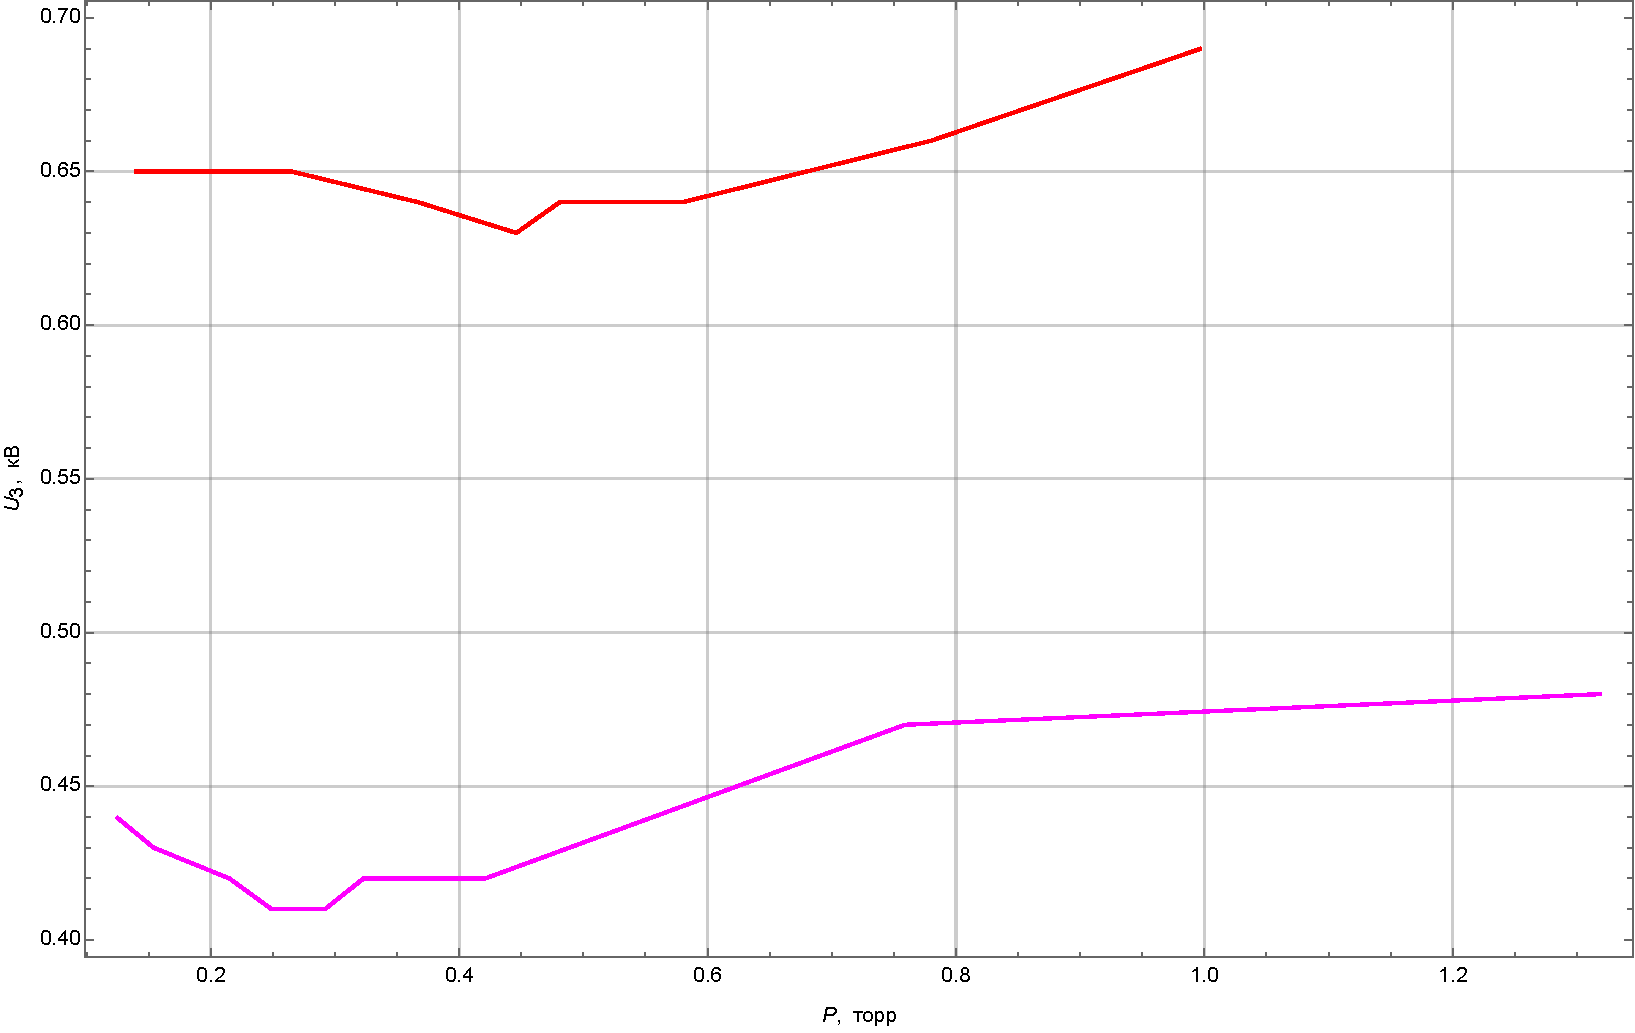
\includegraphics[scale=0.4]{MyGraph5.pdf}
	\caption{Сравнение графиков}
	\label{fig:Graph5}
\end{figure}
\section{Вывод}
Мы рассмотрели самостоятельный тлеющий разряд, сравнили характеристики при разном составе газа в стабиловольте, убедились в верности происходящих физических явлений при тлеющем газовом разряде.
\section{Литература}

\end{document}